\section{Conjunto de datos}

El desarrollo del modelo basado en aprendizaje profundo requiere un conjunto de 
datos apropiado para el entrenamiento. Para poder realizar el pronóstico de 
tormentas eléctricas se utilizarán los datos de densidad de destellos por área 
(Flash Extend Density, FED).

Los datos se encuentran alojados en un bucket de Amazon Web Services, cada 
archivo describe una lista de coordenadas que describe los puntos donde se 
detectaron destellos. Los archivos son generados cada veinte segundos.

Para poder utilizar estos datos, deben representarse en forma matricial, por lo 
que se acumularán en una cuadrícula.

\begin{figure}[H]
  \centering
  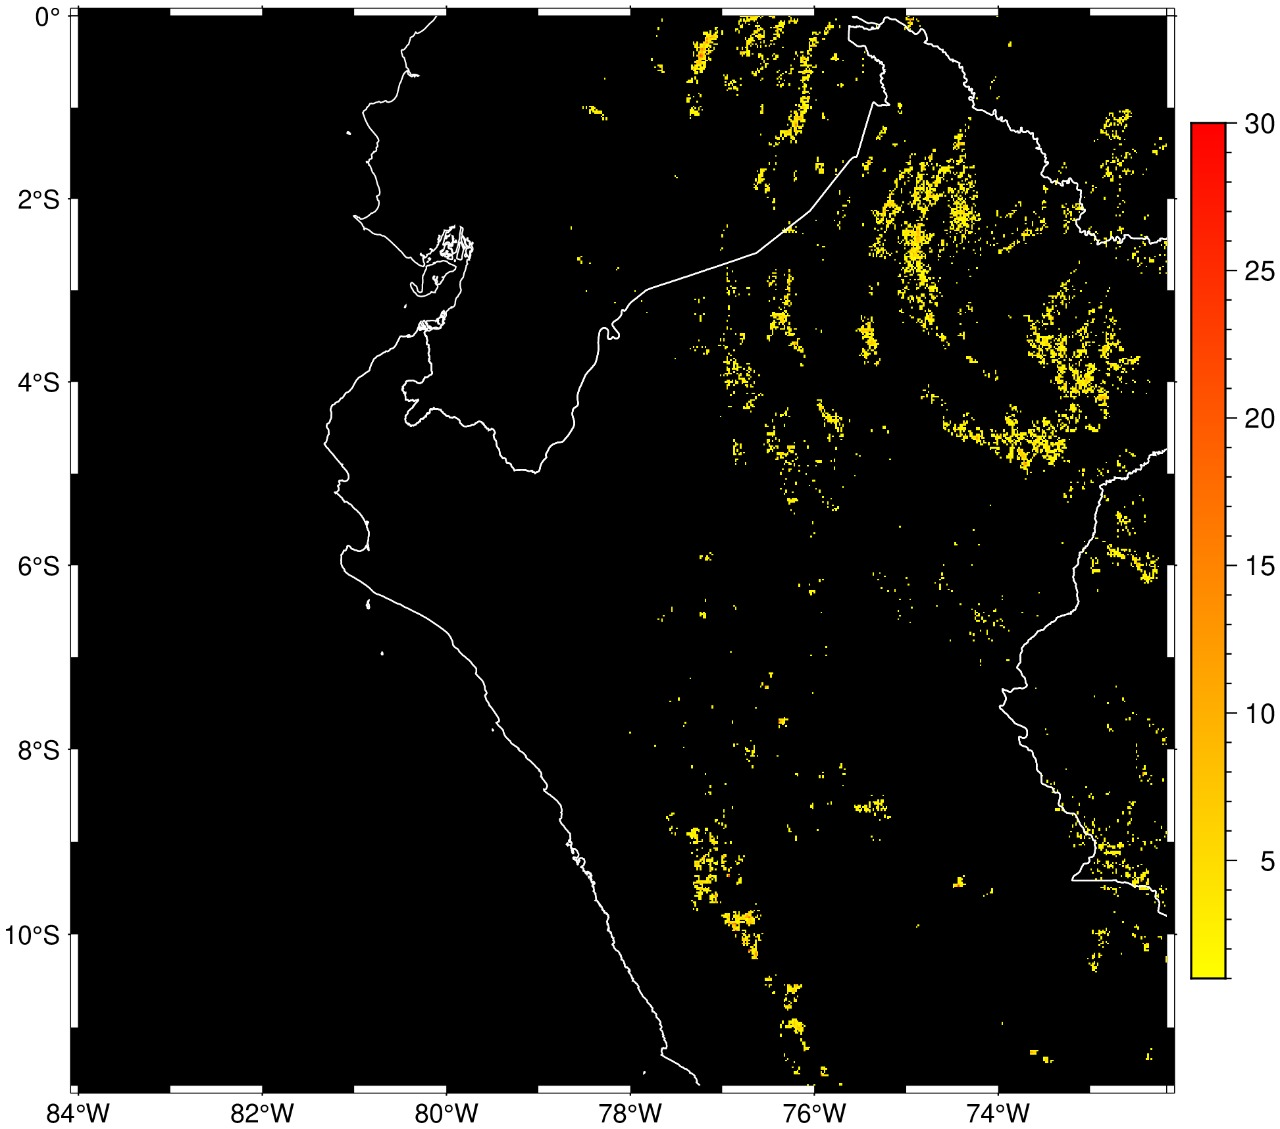
\includegraphics[width=10cm]{E_IMAGENES/5_Metodologia/fed_puntual}
  \caption[Densidad de Destellos por Área]{
    Densidad de Destellos por Área. \newline 
    Fuente: Elaboración propia.
  }
  \label{fig:fed}
\end{figure}



